

\documentclass[runningheads,a4paper]{llncs}

\usepackage{amssymb}
\setcounter{tocdepth}{3}
\usepackage{graphicx}
\usepackage{amsmath}
%\usepackage{amsfonts}
%\usepackage{amsthm}
\usepackage[tight,footnotesize]{subfigure}
%\usepackage{caption} 
%\usepackage{subcaption}
%\usepackage{cite}
\usepackage{hyperref}
\usepackage{url}
\usepackage{clrscode4e}
\urlstyle{same}
\newcommand{\keywords}[1]{\par\addvspace\baselineskip
\noindent\keywordname\enspace\ignorespaces#1}

\makeatletter
\let\c@lemma=\c@theorem
\let\c@corollary=\c@theorem
\let\c@fact=\c@theorem
\makeatother

\let\realendproof=\endproof
\def\endproof{\hspace*{\fill}$\Box$\realendproof}


\begin{document}

\mainmatter  

\title{Experiments on ANTS Algorithms Without Communication}
\author{Fermi Ma \and Nicolas Rakover \and Erik Waingarten}
\institute{MIT}

\maketitle

\section{Introduction}

We study the \emph{Ants Nearby Treasure Search} (ANTS) problem for modelling collective foraging in animal groups. $k$ identical probabilistic agents search for treasure located by an adversary $D$ units away from a central location. The problem is a generalization of a previously studied problem, the \emph{cow-path} problem, which is the case where $k = 1$. 

Our project is a combination of a reading project and an experimental project. For the reading project component, we survey three known algorithms for the ANTS algorithm by Feinerman et al. and Lenzen et al. For the experimental project, we show the results of tests run on these algorithms to determine the constants in their runtimes.

The paper is organized as follows. In Section~\ref{problem statement}, we formally state and motivate the problem. We also give a simple argument for why any algorithm solving the problem takes $\Omega(D+D^2/k)$ time. We then outline different algorithm types, and give high-level overviews of the spiral, harmonic, and lines algorithms. In Section~\ref{spiral}, we give a more in-depth explanation of the details of the spiral algorithm of Feinerman et al. We do this for the harmonic algorithm in Section~\ref{harmonic}, and for the lines algorithm in Section~\ref{lines}. In Section~\ref{experiments}, we shift our focus to the experimental part of our project. In that section, we describe our hypotheses, our experimental setup, the results, and our interpretation of the results. We give concluding remarks in Section~\ref{conclusion}. 

\section{Problem Setup and Basics}
\label{problem statement}

There are $k$ mobile agents searching for treasure in the two-dimensional grid $G$ with vertex set $\mathbb{Z}^2$. All $k$ agents start the search from a central \emph{source} node $s \in G$. An adversary places the treasure at some target node $\tau \in G$ at a \emph{hop distance} $D$ away from $s$. The hop distance is the minimum number of grid edges that must be traversed to get from one node to another, and is also known as the taxicab distance. We denote the hop distance from the starting node $s$ to some point $t$ as $d(t)$. The goal of the agents is for one of them to find the treasure by reaching the node $\tau$.

It is assumed that the agents act synchronously, and that they all start their search at the same time $t_0$. Each edge traversal costs one unit of time, so the total time (or cost) it takes to run an algorithm is the number of edges traversed by the first agent to find the treasure. The cost of a given algorithm $\mathcal{A}$ is the expected time it takes to find the treasure, which is denoted by $T_\mathcal{A}(D,k)$.

\subsection{A Simple Lower Bound}

There is a simple $\Omega(D+D^2/k)$ lower bound which follows from the following argument. The time it takes $T$ for an algorithm to run must satisfy $T \geq D$, or else it is not even possible to reach treasure $D$ units away. 

Also, $T$ must satisfy $T \geq D^2/4k$. To see why, suppose not. Then $T < D^2/4k$, and in particular $2kT < D^2/2$. Thus, out of all the points that are at most $D$ away from the source $s$, by time $2T$, strictly less than half of them have been visited. This implies that some node at most $D$ units away is visited with probability less than $1/2$ by time $2T$. If the adversary simply places the target at that node, then the expected time to find the treasure is strictly greater than $T$, which is a contradiction.

Note this lower bound holds even if the agents knows the total number of agents. 

\subsection{Types of Algorithms}
We will focus on three kinds of algorithms:
\begin{itemize}
\item Spiral algorithms
\item Lines algorithms
\item Harmonic search algorithm
\end{itemize}

And each algorithm has two flavours: \emph{uniform} and \emph{non-uniform}. We say that an algorithm is non-uniform in parameter $p$ if $p$ is an input to the algorithm. If the parameter $p$ is not an input, then the algorithm is uniform in $p$. 

For example, a spiral algorithm which is non-uniform in $k$ is the algorithm where agents can know how many total agents there are. An algorithm which is non-uniform in $D$ has an upper bound on the hop distance of the treasure. 

The spiral and Harmonic search algorithms are similar strategies and were introduced by \cite{feinerman2012collaborative}. Both rely on the ``spiral" procedure, in which an agent covers a space of $\sqrt{d}$ grid cells in $O(d)$ time. Figure~\ref{fig:spiral} shows a possible spiral routine.
There will be two kinds of spiral algorithms, non-uniform in $k$ and uniform in $k$. There will be three kinds of lines algorithms, non-uniform in $D$, non-uniform in $k$, and uniform in both $k$ and $D$. The Harmonic search algorithm is extremely simple and uniform in both $k$ and $D$. 

\begin{figure}
\centering
\label{fig:spiral}
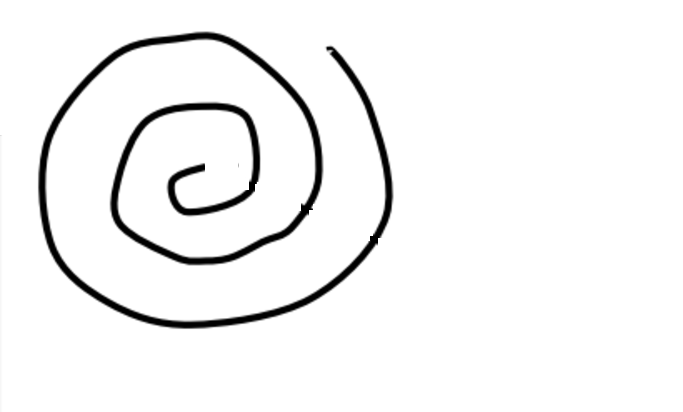
\includegraphics[width=0.4\linewidth]{justspiral.pdf}
\caption{Possible spiral, covering $\sqrt{d}$ grid cells in $O(d)$ time}
\end{figure}

\section{Spiral Algorithms}
\label{spiral}

The following short explanations are from \cite{feinerman2012collaborative}.

\subsubsection{Non-uniform in $k$}

Given the number of agents taking part in the search, we could imagine an algorithm in which the grid in divided into $k$ parts, similar to a pizza being divided into $k$ equal parts. Each agent could cover his portion, and this would yield an asymptotically optimal algorithm. However, this assumes that the agents can communicate with each other and decide which portion belongs to which agent. 

In order to get around this, we can introduce some randomization. If each agent picks a random grid cell within some distance $D$, travels to that distance and performs a spiral of sufficiently large size, it can expect that all agents together will search new areas. If we repeat this sufficiently many times, we can expect that the whole area within distance $D$ was covered. Then we just need to estimate the value of $D$.

This is what the spiral algorithms does when its non-uniform in $k$. 

\begin{codebox}
\Procname{Each agent performs the following double loop}
\li \For $j$ from $1$ to $\infty$, \Then
\li \For $i$ from $1$ to $j$ \Then
\li Go to a node chosen uniformly at random from nodes a distance $2^{i}$
\li Perform a spiral search for $2^{2i+2}/k$ steps
\li Return to source \End \End 
\end{codebox}

We provide a sketch of the proof to show the algorithm has expected running time $O(D + D^2/k)$. Note that the time until agents reach some value of $j$ is $O(2^j + 2^{2j}/k)$. Also, note that once $i \geq \log D$, the spiral will intersect the ball of radius $D$ significantly, and so the probability that an agent finds the treasure is some constant $\beta$. Therefore, the probability that no agents find it after $l$ phases of $i$ is $(1 - \beta/k)^{kl}$, which is also at most some constant probability $\gamma$.

So for each additional $l$ values of $j$ once $j = \lceil \log D \rceil$, there are $l^2/2$ phases where $i \geq \log D$, and so the probability that a round takes $O(2^{j + l} + 2^{2(j+l)}/k)$ is $\gamma^{l^2/2}$, and so in the computation of the expected value, the sum of all $l$ converges to some constant. And we are left with a runtim of $O(2^{j} + 2^{2j}/k)$ for $j = \log D$. This finishes the sketch.

\subsubsection{Uniform in $k$}

Once we have the spiral algorithm non-uniform in $k$, we can make it uniform in $k$ by successively doubling estimates of $k$. This means that at each stage, we take a guess of what $k$ is, and we simulate the algorithm. There is some additional bookkeeping to ensure that enough iterations are made, but the optimization is similar. There is higher lower bound on how fast these algorithms can run, and we get a multiplicative factor of $f(\log k)$, where $f$ is a function such that $\sum \dfrac{1}{f(n)}$ converges. There is a corresponding lower bound that shows this algorithm is asymptotically optimal.

\section{Harmonic Algorithm}
\label{harmonic}

The following is a brief explanation of the Harmonic search algorithm, which, as mentioned earlier, is uniform in both $k$ and $D$.

The main idea is to avoid maintaining a state associated with an estimate of $D$ by randomly regions in the plane such that smaller $D$ will be explored earlier more often. More specifically, the procedure as presented in \cite{feinerman2012collaborative} is composed of the following three steps, performed indefinitely: (1) choose a random direction and walk a distance $d$ in that direction from the source, where $d$ is sampled with probability approximately inversely proportional to $d$, (2) do a spiral search for time $\sim d^2$, and (3) return to the source.

The expected performance of the algorithm is determined by a fixed value $\delta > 0$. The formal description of the algorithm, shown below, uses the probability distribution $p(u) := \frac{c}{d(u)^{2+\delta}}$, where $u$ is a point in the plane, $d(u)$ the distance from the source to $u$, and $c$ a normalizing factor. The following is performed by each agent:

\begin{codebox}
\li \textbf{begin}
\Then 
\li Go to node $u$ with probability $p(u)$
\li Perform spiral search for time $t(u) := d(u)^{2+\delta}$
\li Return to source 
\End
\li \textbf{end} 
\end{codebox}

The performance guarantees of the algorithm are stated formally below. For a proof of the statement, please refer to \cite{feinerman2012collaborative}: \\

\emph{
Let $\delta \in (0,0.8]$. For every $\epsilon > 0$, there exists a positive real number $\alpha$ such that if the number $k$ of agents is greater than $\alpha D^{\delta}$, then with probability at least $1-\epsilon$, the expected running time of the harmonic algorithm is $O( D + \frac{D^{2+\delta}}{k})$.
}

\section{Lines Algorithm}
\label{lines}

The lines algorithm is the study of \cite{lenzen2014trade}, where they cover a lines algorithm which is non-uniform in $D$ and non-uniform in $k$. We use the ideas of \cite{feinerman2012collaborative} to design a lines algorithm which is uniform in both $k$ and $D$. The lines algorithm has many optimizations since \cite{lenzen2014trade} are trying to reduce \emph{selection complexity}. Selection complexity is a metric which measures how likely an algorithm is to occur naturally in nature. Of course, this notion is very vague, but formally, the selection complexity $\chi$ of an algorithm $A$ is $\chi(A) = b + \log l$ where $b$ is the amount of memory usage and $l$ is smallest $l$ for which the algorithm does not need finer probabilities than $2^{-l}$. In \cite{lenzen2014trade}, Lenzen et al. provided a lines algorithm with selection complexity $O(\log \log D)$.

\subsubsection{Non-uniform in $D$} First, we will explain the simple lines algorithm which is non-uniform in $D$. Remember, $D$ is an upper bound on the distance the treasure. The lines algorithm is very simple to explain. With probability $\frac{1}{2}$, an agent moves up, otherwise, it moves down. Then it continues moving in that direction until a coin with head probability $\frac{D-1}{D}$ lands on tails. It repeats the process for the left and right directions. The pseudocode is shown, $C_p$ will denote a coin which lands heads with probability $p$, and so $C_p$ will return a 0 or 1, with 0 denoting heads.

The algorithm relies on it novel way of walking in lines by approximately counting. The following procedure shows how an agent would move in a particular direction. 

\begin{codebox}
\Procname{moveDirection(dir)}
\li \While $C_{\frac{D-1}{D}} = 0$ \Then
\li agent moves in direction dir \End
\end{codebox}

Note that the above algorithm, while it uses contant memory, it does need to sample from a distribution with probability as fine as $\frac{1}{D}$. This is fine, since in this case, $l = \log D$. 
Now that we know how agents move in a particular direction, they randomly pick a direction to travel.

\begin{codebox}
\Procname{Each agent performs the following iteration}
\li dir[0] $\leftarrow$ up, dir[1] $\leftarrow$ down
\li $i \leftarrow C_{\frac{1}{2}}$
\li moveDirection($i$)
\li \If $C_{\frac{1}{2}} = 0$ \Then
\li moveDirection(left)
\li \Else moveDirection(right) \End \End
\li return to origin
\end{codebox}

The one thing to note is that the last line, ``return to origin" would need to keep the location of the ant. This would require $\log D$ memory, which we cannot afford; however, it is an assumption in the model that agents can return to the origin.

% TO DO
The sketch of the proof of correctness is the following ...????

\subsubsection{Uniform in $D$}

\section{Experiments and Results}
\label{experiments}

In this section, we show our results for the experiments we ran on the algorithms mentioned above. We do not go into detail regarding the various implementations of the algorithms, but all of the code, along with the data used is available online hosted in the git repository: \url{https://github.com/erikwaing/6.852-Ants.git}. 

We implemented the three algorithms, in the possible different uniformity flavours. Even though \cite{lenzen2014trade} does not go into detail on how to make the Lines algorithm uniform in $k$, we apply the same techniques as in \cite{feinerman2012collaborative}. This allows us to compare the algorithms on an equal setting, with both non-uniform in $k$ and uniform in $k$ flavours. 

In the Lines algorithm, there are optimizations made in order to keep memory low. For example, in the outer loop of the Lines algorithm which is uniform in $D$, but not in $n$, there is some approximate counting. We note that the algorithm still works with the same runtime if instead of the approximate couting, we looped for as long as the expected value of the number of loops. This keeps the expected runtime the same, and decreases the variance runtime, which will allow us to converge to constants experimentally quicker. These approximate countings were made in order to optimize memory, and we are only focused on the runtime of the algorithms.

\subsubsection{Experimental Setup}

We had to run the Spiral algorithm and the Lines algorithm differently from the Harmonic Search algorithm. This is because the Harmonic Search requires arbritrary fine probabilites. The technique we used for implementing the Harmonic Search relies on sampling uniformly from the interval $(0, 1)$, and then applying some transformations. Since we implemented the algorithm in python, and used \texttt{random.random()} in order to sample uniformly from $(0,1)$, we are limited by the granurality of the python module. This means that our current implementation of the Harmonic Search has an upper bound on how far $D$ can be. We believe finding better ways to implement this algorithm is an interesting research direction, both in the theoretical algorithms world, as well as the experimental algorithms world. 

For testing the Lines and Spiral algorithms, we ran the following series of experiments. 
\begin{enumerate}
\item We set $D = 40$, and left it at 40 for the whole experiments. 
\item We vary $k$ from $10$ to $200$ inclusive in intervals of 10. 
\item We run each algorithm with each value of $k$ for 100 iterations.
\item We run the experiments on a random placement of the treasure within hop distance $D$ from the origin, which is our source.
\end{enumerate}

For the Harmonic Search algorithm, we were only able to test it for $D = 10$, since for higher values of $D$, the algorithm became prohibitively expensive. We varied $k$ from 10 to 200 inclusive in intervals of 10 as with Lines and Spiral, and we tested each for 100 times, with randomly placed treasures. For the Harmonic Search algorithm we let $\delta = 1$. For the Lines algorithm, we let $K = 6$.  

When done with all the iterations, we compute the average time per 100 experiments and assume that this is the expected value. 

\subsubsection{Hypothesis} We hypothesized that the Lines algorithm will be worse, it terms of runtime, compared to the Spiral algorithm. This stems from the fact that the Lines algorithm is optimizing for selection complexity, which would lead to an algorithm that relies on more randomization and iteration. In fact, in the proof of correctness of the Lines algorithm, many times, the proofs use the asymptotics to engulf some smaller order terms.

\subsection{Findings}

After running the experiments on all six algorithms (Spiral non-uniform in $k$, Spiral uniform in $k$, Lines non-uniform in $D$, Lines uniform in $D$, but not in $n$, Lines uniform in $n$ and $D$, and Harmonic Seach). 

\subsubsection{Non-uniform in $k$} For non-uniform in $k$ algorithms, we assume that the expected runtime of the algorithms is given by the following formula
\[ E[T] = c_1 + c_2 / k \]
Where we are keeping $D = 40$. So we are looking to compute the constants $c_1$ and $c_2$ for the Spiral and Lines algorithm. Figure~\ref{nonuniformresultsone} and Figure~\ref{nonuniformresultstwo} shows the $k$ being graphed against $k * E[T]$, which we expect to be linear with solve $c_1$ and intercept $c_2$. Using linear regression, we are able to estimate the values of $c_1$ and $c_2$. 
\begin{center}
\begin{tabular}{l | c c}
\text{Algorithm} & $c_1$ & $c_2$ \\
\hline
\text{Spiral} 	   &147 & 21567 \\
\text{Lines}	   & 896 & 32730 
\end{tabular}
\end{center}

\begin{figure}
\centering
\label{nonuniformresultsone}
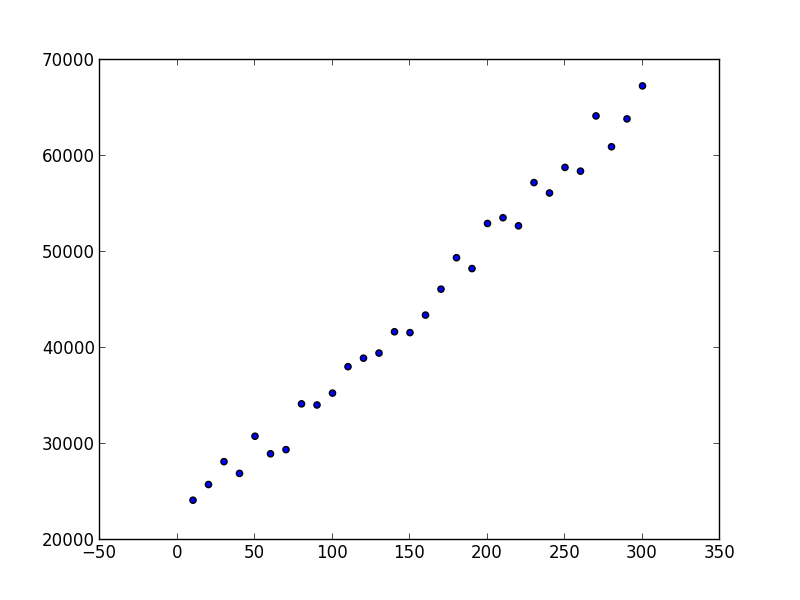
\includegraphics[width=0.5\linewidth]{FKLS1.png}
\caption{Spiral algorithm non-uniform in $k$, $kE[T]$ is the $y$-axis and $k$ is in the $x$-axis}
\end{figure}

\begin{figure}
\centering
\label{nonuniformresultstwo}
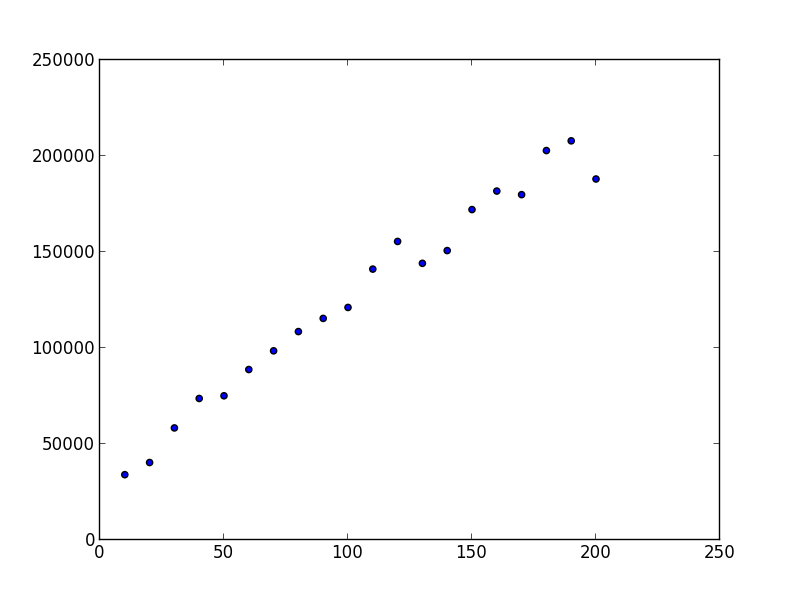
\includegraphics[width=0.5\linewidth]{LinesUniformInD.png}
\caption{Lines algorithm non-uniform in $k$, $kE[T]$ is the $y$-axis and $k$ is in the $x$-axis}
\end{figure}

\subsubsection{Uniform in $k$} For uniform in $k$ algorithms, we assume that the expected runtime of the algorithms is given by the following formula
\[ E[T] = f(\log k)(c_1 + c_2 / k) \]
Where we set $f(x) = x^2 + 1$. This satisfies all our constraints from the theorems in the paper.
Again, we keep $D = 40$ and we want to compute the constants $c_1$ and $c_2$ for the Spiral and Lines algorithm. Figure~\ref{uniformresultsone} and Figure~\ref{uniformresultstwo} shows the $k$ being graphed against $k * E[T]/f(\log k)$, which we expect to be linear with solve $c_1$ and intercept $c_2$. Using linear regression, we are able to estimate the values of $c_1$ and $c_2$. 
\begin{center}
\begin{tabular}{l | c c}
\text{Algorithm} & $c_1$ & $c_2$ \\
\hline
\text{Spiral} 	   &222 & 19954 \\
\text{Lines}	   & 284 & 76762 
\end{tabular}
\end{center}

\begin{figure}
\centering
\label{uniformresultsone}
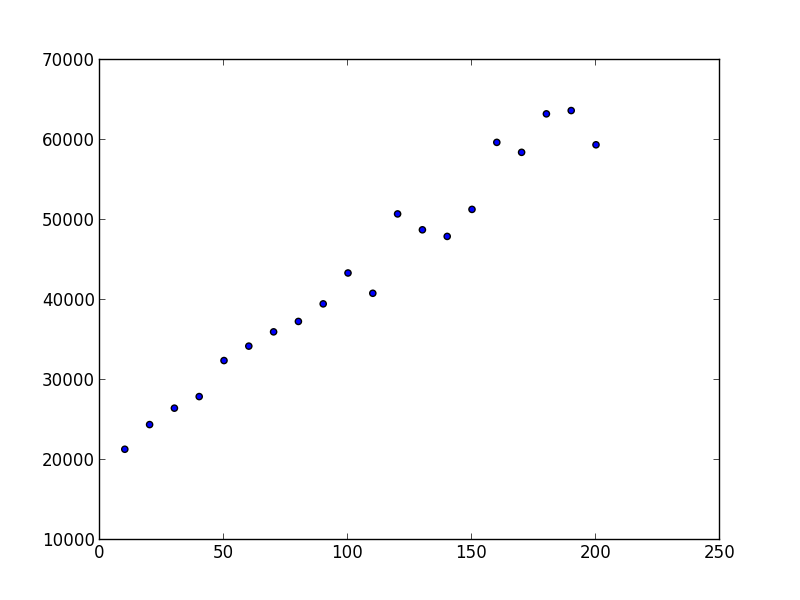
\includegraphics[width=0.5\linewidth]{FKLS2.png}
\caption{Spiral algorithm uniform in $k$, $kE[T]/f(\log k)$ is the $y$-axis and $k$ is in the $x$-axis}
\end{figure}

\begin{figure}
\centering
\label{uniformresultstwo}
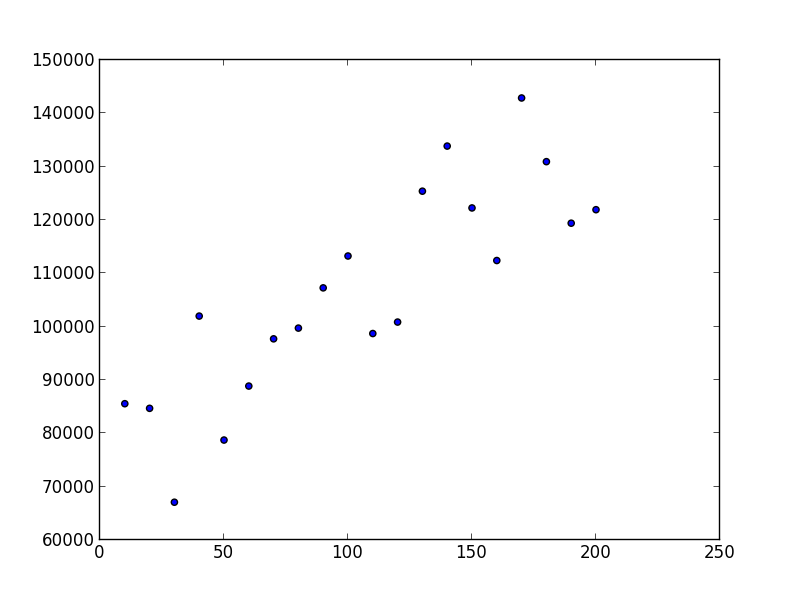
\includegraphics[width=0.5\linewidth]{LinesUniformInAll.png}
\caption{Lines algorithm non-uniform in $k$, $kE[T]/f(\log k)$ is the $y$-axis and $k$ is in the $x$-axis}
\end{figure}

\subsubsection{Interpretation}
This shows that in fact, when only analyzing runtime. The Spiral algorithm performs better than the Lines algorithm in both uniform and non-uniform cases. This of course, was expected, since the Lines algorithm optimizes for memory. 

Some interesting thing we noted is that when running the Lines algorithm in the non-uniform flavour in $D$, we noted that there were lower order terms which were important in the runtime. Figure~\ref{nonuniforminD} and Figure~\ref{nonuniforminDtwo} show how there are lower order terms that are hidden in the asymptotics that do make a difference in the experiments for small $k$. In fact, the assumption that $E[T] = c_1 + c_2 / k$ gives us the graph Figure~\ref{nonuniforminD} being a line, whereas the assumption $E[t] = c_1/ k + c_2 / k^2$ gives us the graph Figure~\ref{nonuniforminDtwo} being a line, which is much more accurate.

\begin{figure}
\centering
\label{nonuniforminD}
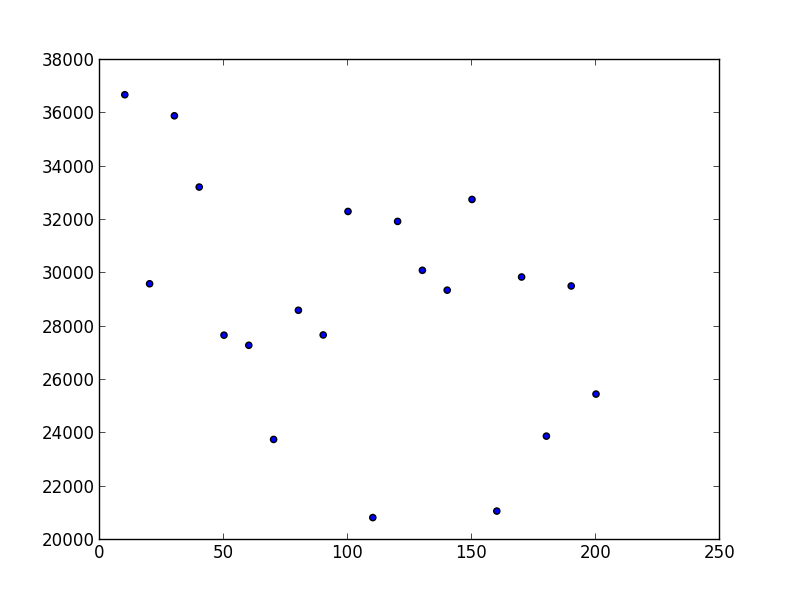
\includegraphics[width=0.5\linewidth]{LinesNonUniformnT.png}
\caption{Lines algorithm non-uniform in $D$, $kE[T]$ is the $y$-axis and $k$ is in the $x$-axis}
\end{figure}

\begin{figure}
\centering
\label{nonuniforminDtwo}
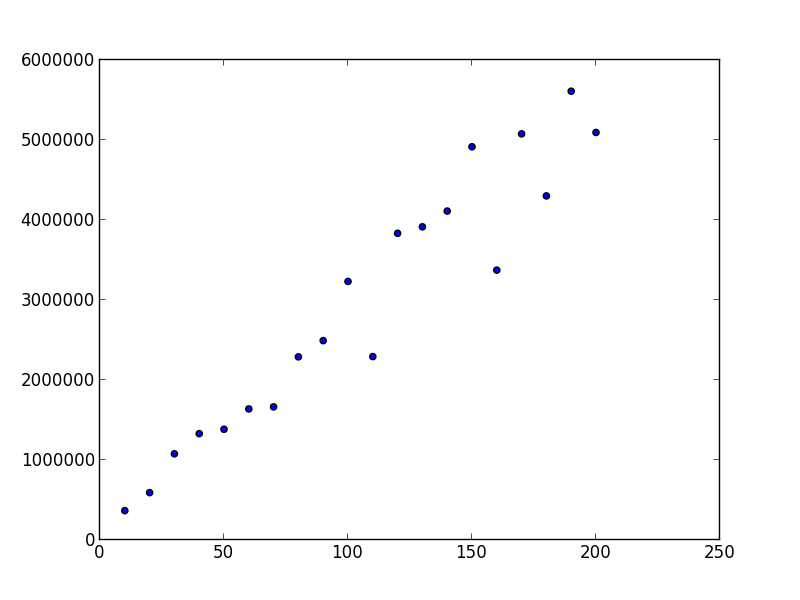
\includegraphics[width=0.5\linewidth]{LinesNonUniformn2T.png}
\caption{Lines algorithm non-uniform in $D$, $k^2E[T]$ is the $y$-axis and $k$ is in the $x$-axis}
\end{figure}

\subsection{Harmonic Search}

We assume that the expected value for the runtime of the Harmonic Search algorithm is given by the following formula
\[ E[T] = c_1 + c_2 / k \]
and we compute the constants $c_1$ and $c_2$. We get that for $D=10$, $c_1 = 148$ and $c_2 = 2319$. Figure~\ref{harmonic}

\begin{figure}
\centering
\label{harmonic}
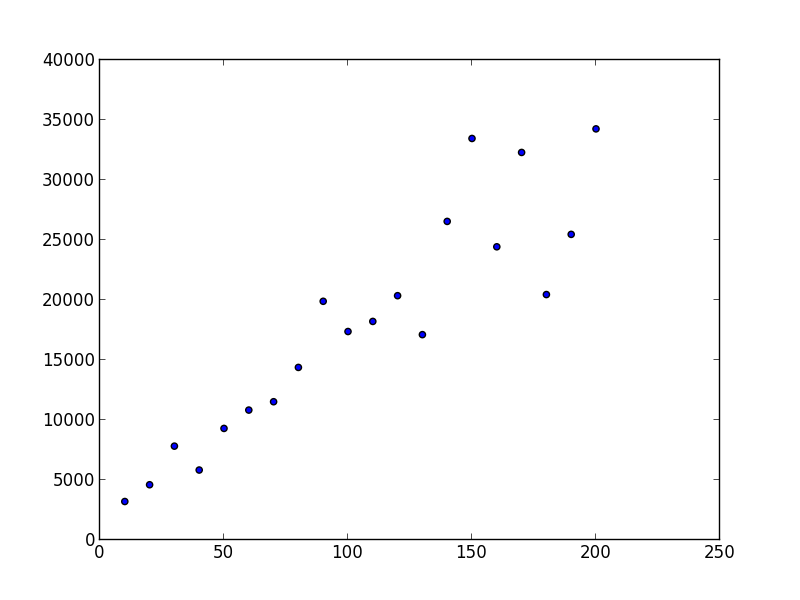
\includegraphics[width=0.5\linewidth]{Harmonic.png}
\caption{Harmonic Search algorithm, $kE[T]$ is the $y$-axis and $k$ is the $x$-axis.}
\end{figure}

\section{Conclusion}
\label{conclusion}

In this paper, we have surveyed the recent literature on the Ants Nearest Treasure Search problem, and have identified three prominent algorithms: the spiral algorithm, the harmonic algorithm, and the lines algorithm. For each algorithm, we considered cases where they are either uniform or not uniform in the variables $D$ and $k$. The lines algorithm was motivated by the idea of a selection complexity, a parameter that roughly models how complex a certain algorithm is. While the spiral and harmonic algorithms achieved good / optimal asymptotic bounds, the lines algorithm could do so while maintaining a low (favorable) selection complexity.

Due to the relative simplicity of the lines algorithm, we conjectured that the good asymptotic runtime of the lines algorithm was hiding its costs in constant factors. We ran experiments comparing the three algorithms with each other, which confirmed our intuition that the lines algorithm had the worst actual runtimes. In fact, it turned out that the lines algorithm had a large $O(1/k^2)$ term that did not show up in the asymptotics, but mattered for the values of $k \leq 200$ that we tested. We claim that these $k$ are worth considering, as many real ant colonies such as those made by acorn ants can have $k$ values of that size.

Our work leaves some questions unresolved, and given more time, we would have liked to pursue some of these lines of inquiry. One question that we would like to know is what the exact values of constants are as we vary the parameter $D$. Another issue we had was that when we performed simulations of the harmonic search algorithm, we did not have a good way of sampling from the theoretical probability distribution. Improving this sampling technique would increase the accuracy of our results. Finally, we would like to consider the problem of placing treasure in an adversarial sense. Note that when we randomly place treasure, as we did in simulations, the question is how long it takes for us to find this random treasure in expectation. When we adversarially place treasure at distance $D$, it is assumed that the treasure is the last distance $D$ square the ants reach, so the problem is simply to fully cover an area of space. We wonder how considering adversarial placement of treasure would impact our results.

\bibliographystyle{plain}
\bibliography{references}

\end{document}
